
\section{Limite e Continuidade}

Seja $f:D\subset\R^2\to \R$ uma função cujo domínio contém pontos arbitrariamente próximos de {\color{blue}$(a,b)$}. Usamos a notação 
\[\lim_{(x,y)\to {\color{blue}(a,b)}}f(x,y)={\color{red}L},\]
para indicar que os valores de $f(x,y)$ se aproximam do número {\color{red}$L$} quando o ponto $(x,y)$ se aproxima do ponto {\color{blue}$(a,b)$} ao longo de qualquer cominho contido no domínio da função $f$.


\begin{definb}{}{} 
Seja $f:D\subset\R^2\to \R$ uma função cujo domínio contém pontos arbitrariamente próximos de {\color{blue}$(a,b)$}. Dizemos que {\color{blue} o limite de $f(x,y)$ quando $(x,y)$ tende a $(a,b)$} é o número {\color{blue}$L$}, e escrevemos
\[\lim_{(x,y)\to {\color{blue}(a,b)}}f(x,y)={\color{red}L},\]
quando para cada $\varepsilon>0$, existe $\delta>0$ tal que
\begin{center}
se $\|(x,y)-{\color{blue}(a,b)}\|<\delta$, então $|f(x,y)-{\color{red}L}|<\varepsilon$.
\end{center}
\end{definb} 

\begin{center}
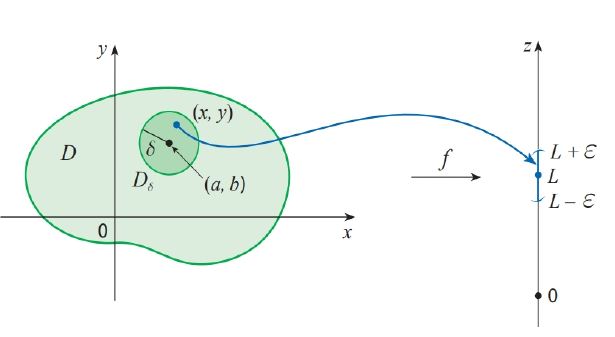
\includegraphics[scale=0.7]{figuras/limite1.png}

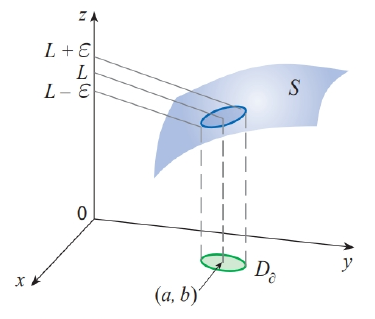
\includegraphics[scale=0.7]{figuras/limite2.png}
\end{center}
\newpage


\begin{caixaazul}{}
Todas as propriedades de limites de funções  de uma variável se estendem às funções de várias variáveis. Por exemplo, o limite da soma, diferença, produto ou quociente é a soma, diferença, produto ou quociente dos limites, respectivamente, contanto que esses limites existam e que os denominadores não se anulem.
\end{caixaazul}

\begin{exeb}{}{} Calcule 
\[\lim_{(x,,y)\to(-1,2)}\left(2x^2y-\frac{3y^2}{x+y}\right).\]
\end{exeb}

\vfill

\marcador{subsection}{Mostrando que o limite não existe}

Quando o limite de uma função {\color{blue}existe} em um ponto, então o limite tem que ser {\color{blue}o mesmo ao longo de todos os caminhos} que se aproximam do ponto. 
\smallskip 

No plano podemos nos aproximar de um ponto {\color{blue}$(a,b)$} por {\color{red} um número infinito de caminhos}, assim se existem dois caminhos diferentes tais que $f(x,y)$ tende a valores distintos, então o limite não existe.


\begin{center}
	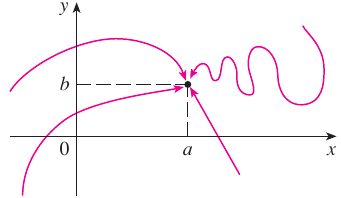
\includegraphics[scale=1]{figuras/lim-caminhos.png}
\end{center}
\newpage


%---------------- exemplo ------------------------------
\begin{exeb}{}{} Mostre que o seguinte limite {\color{red}não existe}
	\[\lim_{(x,y)\to(0,0)}\frac{x^2-y^2}{x^2+y^2}.\]
\end{exeb}  

\begin{center}
	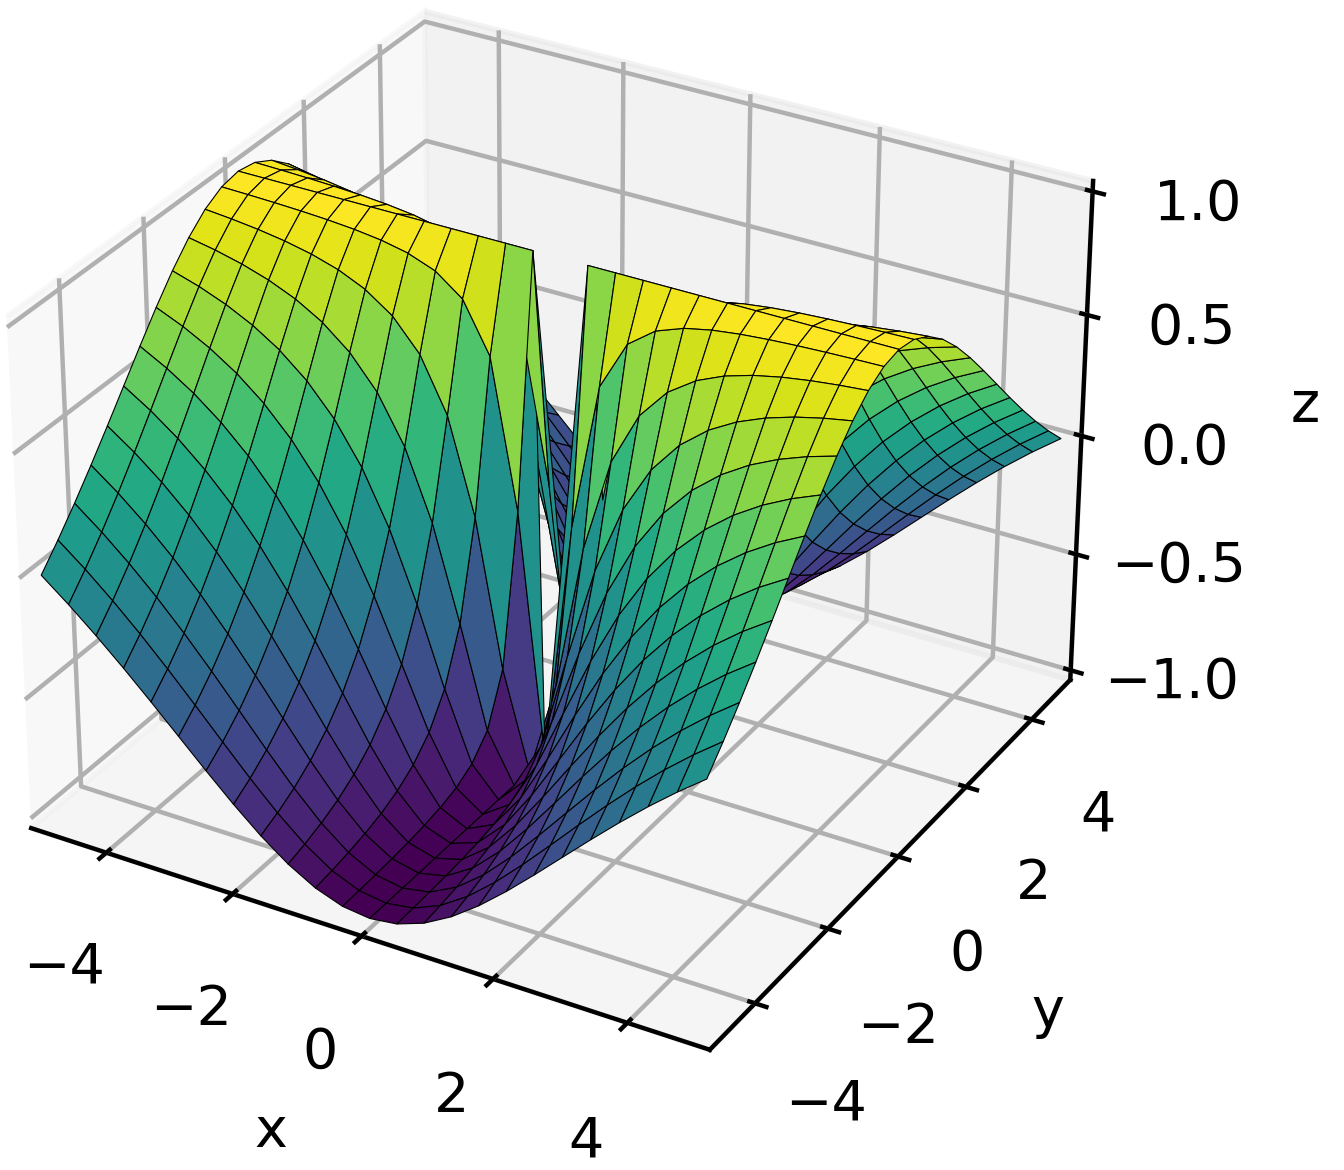
\includegraphics[scale=1]{figuras/lim1.png}
\end{center}
\newpage

%---------------- exemplo ------------------------------
\begin{exeb}{}{}
	Mostre que o seguinte limite {\color{red}não existe}
	\[\lim_{(x,y)\to(0,0)}\frac{xy}{x^2+y^2}\]
\end{exeb}

\begin{center}
	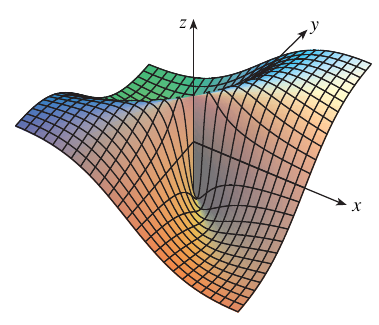
\includegraphics[scale=1]{figuras/lim2.png}
\end{center}

\newpage

%---------------- exemplo ------------------------------
\begin{exeb}{}{}
Mostre que o seguinte limite {\color{blue}existe}
\[\lim_{(x,y)\to(0,0)}\frac{2x^2y}{x^2+y^2}\]
\end{exeb}
\begin{center}
	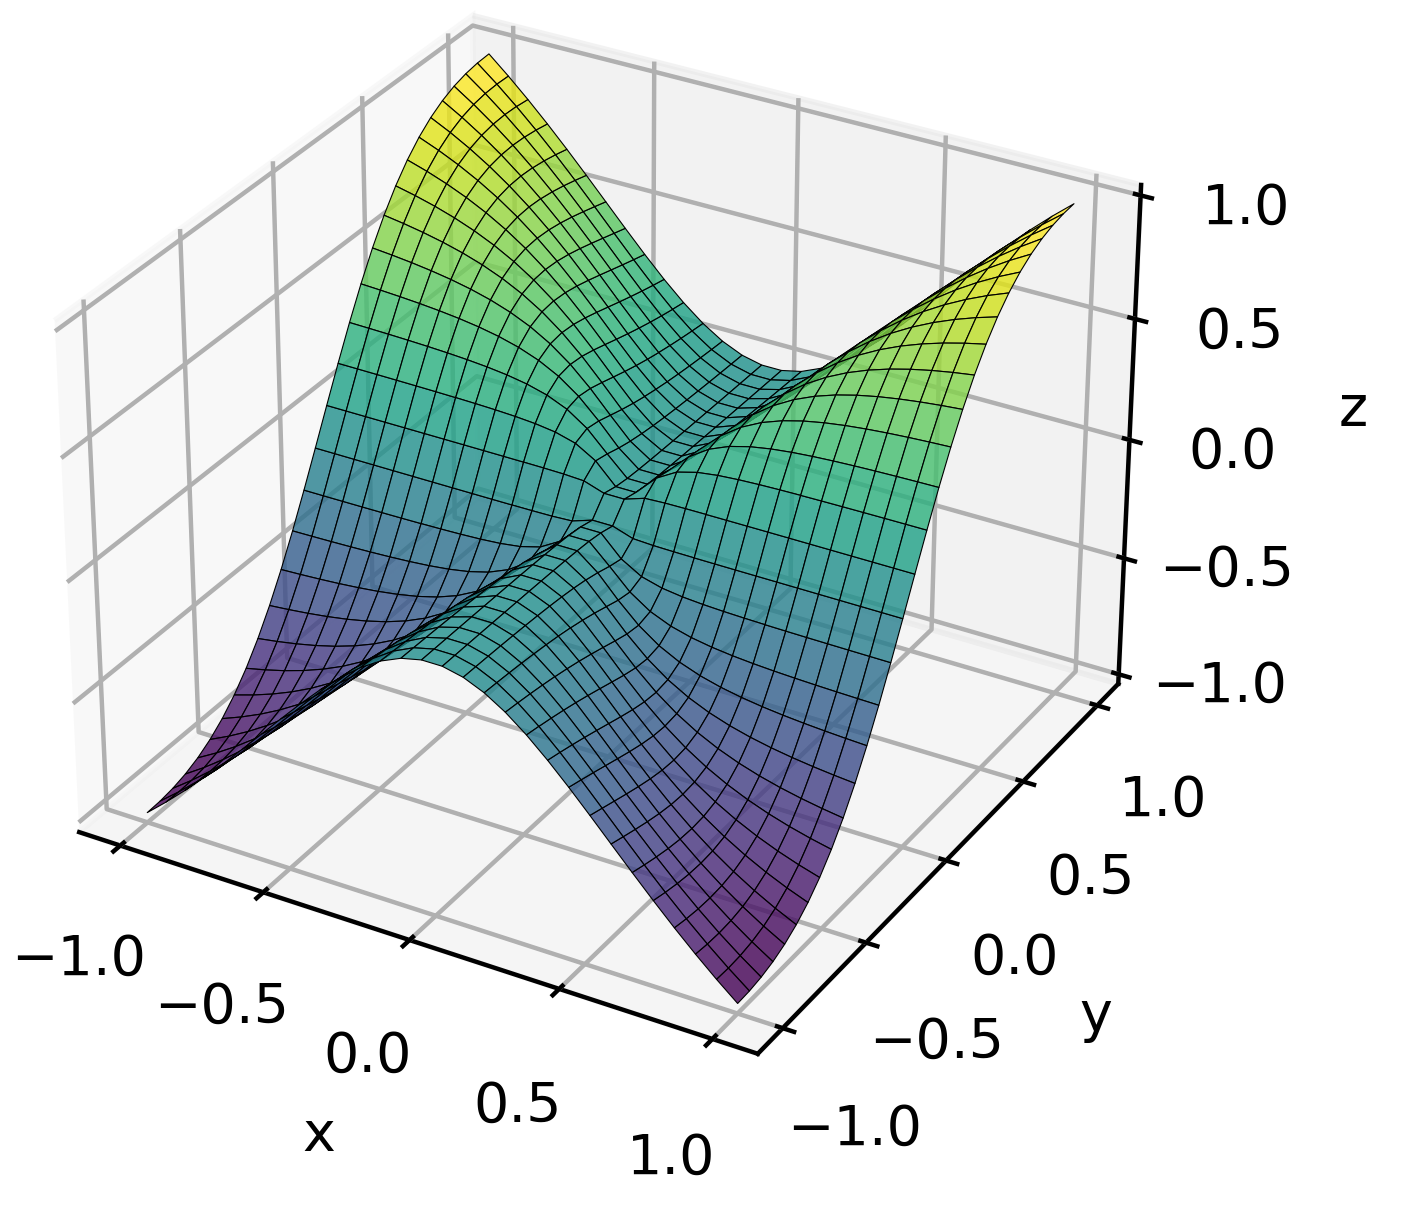
\includegraphics[scale=1]{figuras/lim3.png}
\end{center}		
\newpage

\begin{caixavermelha}{ATENÇÃO!!!}
\begin{itemize}
	\item Mesmo que o limite seja igual para uma infinidade de caminhos, isso não garante que o limite exista!
	\item Basta que ele seja diferente para dois caminhos distintos, para não existir.
	\item Ele só existe quando é o mesmo em todos os caminhos possíveis.
\end{itemize}
\end{caixavermelha}


\begin{exeb}{}{}
	Mostre que o seguinte limite NÃO existe
	\[\lim_{(x,y)\to(0,0)}\frac{xy^2}{x^2+y^4}\]
\end{exeb}
\begin{center}
	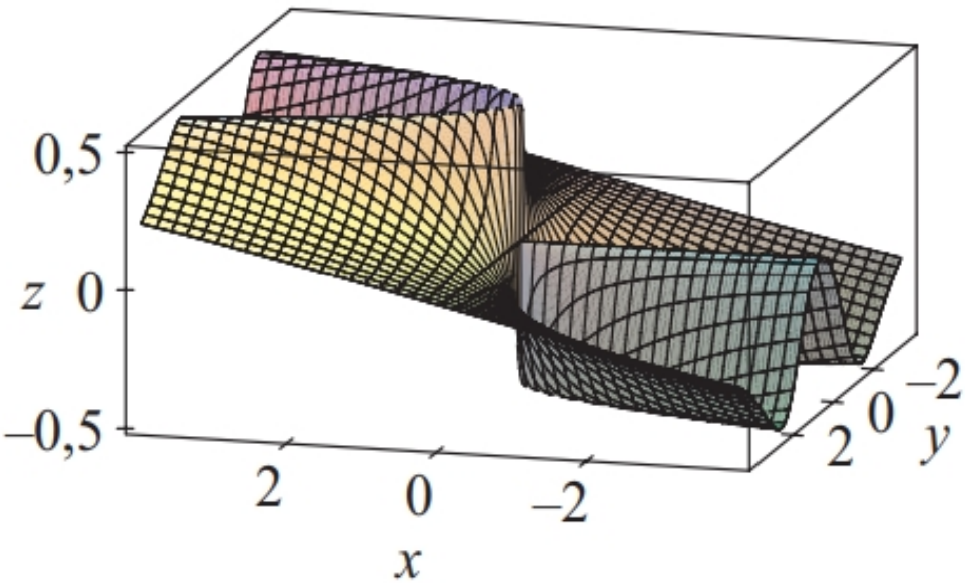
\includegraphics[scale=.5]{figuras/limites/limite-parabola.png}
\end{center}
\newpage

\marcador{subsection}{Continuidade}

\begin{definb}{}{}
 Sejam $f$ uma função real de duas variáveis e {\color{blue}$(a,b)$} um ponto do domínio de $f$. Dizemos que $f$ é \dt{contínua} em $\pz$ se 
$$\lim_{(x,y)\to\pz}f(x,y)=f\pz.$$
Dizemos que $f$ é contínua em $D$ se $f$ é contínua em todos os pontos de $D$.
\end{definb} 

\begin{exeb}{}{}
	
 \begin{enumerate}
\item Funções racionais são contínuas em todos os pontos de seu domínio.
		
		
\item  A função $\arctan\left(\frac{y}{x}\right)$ é contínua em todo o seu domínio pois a composta de funções contínuas também é contínua.
	\end{enumerate}
\end{exeb}

\begin{center}
	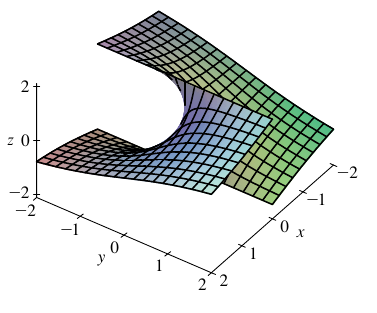
\includegraphics[scale=1]{figuras/cont1.png}
\end{center}

\begin{exeb}{}{}
 Determine os pontos de continuidade de 
\begin{enumerate}

\item $f(x,y)=\left\{\begin{array}{ll}
	\displaystyle\frac{2x^2y}{x^2+y^2}, &(x,y)\neq (0,0)\\
	\\
	0, & (x,y)=(0,0)\\
\end{array}\right.$

\item   $f(x,y)=\left\{\begin{array}{ll}
	\displaystyle\frac{xy}{x^2+y^2}, &(x,y)\neq (0,0)\\
	\\
	0, & (x,y)=(0,0)\\
\end{array}\right.$
\end{enumerate}
\end{exeb} 

Analogamente podemos generalizar estes resultados para funções de mais de duas variáveis quaisquer.
\newpage

\begin{casab}{}{}
\begin{enumerate}
\item Decida sobre a existência do seguinte limite $\displaystyle\lim_{(x,y)\to(0,0)}\frac{x^2y}{x^4+y^2}$.
		
\item Determine os pontos de continuidade da função
		\[f(x,y)=\begin{cases}
		\displaystyle\frac{xy}{x^2+xy+y^2}, & (x,y)\neq (0,0),\\
			0, & (x,y=(0,0).
		\end{cases}\]
		
\item Revise a definição de derivada de função de uma variável $y=f(x)$.
	\end{enumerate}
\end{casab}

